% TODO
%%%%%%%%%%%%%%%%%%%%%%%%%%%%%%%%%%%%%%%%%%%%%%%%%%%%%%%%%%%%%%%%%%%%%%%%%%
\chapter{Hluboký zásobníkový automat v~normální formě} \label{kap_pda_NF}

V~této kapitole zavádím normální formu hlubokého zásobníkového automatu a ukazuji způsob, jakým lze automat na tuto formu převést. Vycházím z~myšlenky automatu s~jedním nevstupním symbolem, kterému jsem se věnovala doposud. Hluboký zásobníkový automat je ale zobecněním konečného a nemá omezení pro počet nevstupních symbolů na zásobníku. Z~toho důvodu není možné na něj aplikovat algoritmus \ref{alg_PDA}, neboť by to vedlo k~nekonečnému počtu stavů a pravidel. Je však možné pracovat podobným způsobem s~tzv. prefixem zásobníku, kdy nejvrchnějších $n$ nevstupních symbolů nahrazuji symbolem $\#$. Celkový počet nevstupních symbolů jsem tak nijak nezredukovala, ale docílila jsem zjednodušeného zápisu pravidel.

% definice
% algoritmus
% ekvivalence



%=========================================================================
\section{Definice normální formy}

Hluboký zásobníkový automat v~normální formě dle definice \ref{def_NF} pracuje s~prefixem $n$ nevstupních symbolů. Přepis symbolů v~prefixu na symbol $\#$ umožňuje pravidlo typu (i), změnu stavu pravidlo typu (ii), přepis na symbol vstupní abecedy pravidlo typu (iii) a expandovat lze pravidlem typu (iv). 

\begin{Def}\label{def_NF}
Nechť $M = (Q,\Sigma,\Gamma, R, s, S~, F)$ je hluboký zásobníkový automat
a $n$ je maximální hloubka expanze v~$M$.
Pak $M$ je v~normální formě, pokud každé pravidlo z~$R$ je v~jednom ze tvarů:

\begin{enumerate}
\renewcommand{\labelenumi}{(\roman{enumi})}

\item $mqA \rightarrow q\#$ pro každé $m$, $q$, $A$ : $1 \le m \le n$, $q \in Q$, $A \in (\Gamma - \Sigma) - \{\#\}$,
\item $mq\# \rightarrow p\#$, kde $1 \le m \le n$, $p$, $q \in Q$,
\item $mq\# \rightarrow pa$, kde $a \in {\Sigma}^+$, $1 \le m \le n$, $p$, $q \in Q$,
\item $mq\# \rightarrow p\#A$, kde $A \in (\Gamma - \Sigma) - \{\#\}$, $1 \le m \le n$, $p$, $q \in Q$.

\end{enumerate}

Nechť pravidlo typu (i) lze aplikovat jen na nejvrchnější možný nevstupní symbol na zásobníku a typ (iv) je možné aplikovat jen na nejspodnější symbol $\#$, pak na zásobníku je v~každém kroku řetězec z~množiny $ ( \Sigma^* \{ \# \} )^k  \Gamma^*$, kde $0 \le k~\le n$. 

\end{Def}


\begin{figure}[ht]
\centering
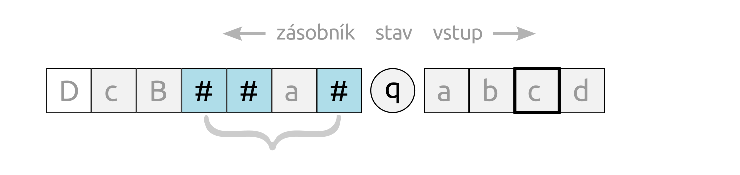
\includegraphics{img/bp_pda04.eps} \bigskip \\
\caption{Příklad konfigurace hlubokého zásobníkového automatu v~normální formě s~prefixem 3.}
\end{figure}

\section{Převod na normální formu}

Při sestavování algoritmu pro převod hlubokého zásobníkového automatu do normální formy jsem musela řešit zejména omezené možnosti expanze. Původní stav automatu a nevstupní symboly z~prefixu opět uchovávám ve stavech. Pokud bych ale připustila expanzi na libovolný počet nevstupních symbolů, ztratila bych ze stavu informaci o~nahrazených nevstupních symbolech, které by se ocitly za prefixem, nebo bych zvětšovala velikost prefixu a počet pomocných stavů by tak narostl do nekonečna. Tento problém jsem vyřešila tzv. postupnou expanzí \cite{Meduna:Theory}. Řetězec na pravé straně pravidla je reprezentován jedním nevstupním symbolem. Ten je možné expandovat na právě dva nevstupní symboly: první symbol v~řetězci a zbývající část řetězce. Jednoduchou rekurzí tohoto postupu lze dosáhnout úplné expanze.

Expanze na dva nevstupní symboly je již udržitelná, ale pokud bych neomezila použití pravidla typu (iv), stále by se mohlo stát, že poslední symbol $\#$ bude odsunut o~jednu pozici za prefix. Nabízelo se povolit pravidlo pro přepis tohoto symbolu na původní nevstupní symbol, ale tím bych zvýšila hloubku automatu. Místo toho spojuji krok expanze a krok přepisu posledního $\#$ symbolu na původní symbol do jednoho pravidla. Expanze tak nemá vliv na $\#$ symboly v~prefixu.

V~algoritmu \ref{alg_NF} popisuji konstrukci hlubokého zásobníkového automatu v~normální formě. S~ohledem na postupnou expanzi zavádím nové nevstupní symboly, jejichž součástí je rovněž původní pravidlo pro expanzi. Nelze určit dopředu, kdy se jednotlivé kroky expanze provedou, proto je nutné umožnit je provést ve všech stavech automatu a na všech pozicích v~prefixu. 
Ukázka aplikace tohoto algoritmu je k dispozici v příkladu \ref{example_NF}.

\begin{Alg}\label{alg_NF}
Převod hlubokého zásobníkového automatu do normální formy.

\begin{list}{}{\setlength\parsep{0cm} \setlength\itemsep{0cm} \setlength\leftmargin{1em}}
   \item Vstup: $M = (Q,\Sigma,\Gamma, R, s, S, F)$ 
   \item Výstup: $M_{NF} = (Q_{NF}, \Sigma_{NF}, {\Gamma}_{NF}, R_{NF}, s_{NF},  S_{NF}, F_{NF})$ \medskip
  
  \item ${\Sigma}_{NF} := \Sigma$
  \item $s_{NF} := <s,S>$
  \item $S_{NF} := \#$ \medskip

  \item $k := \mathrm{max}(\{m \mid mqA \rightarrow pv \in R\}) $ \medskip

  \item Pro každé $(q,u,A) \in Q \times (\Gamma - \Sigma)^* \times (\Gamma - \Sigma)$, kde $|u| < k$: \medskip

  \subitem přidej do $R_{NF}$ pravidlo typu (i) $|uA| <q,u> A~\rightarrow <q,uA> \#$. \medskip

  \item Pro každé $r : mqA \rightarrow p X_1 X_2 X_3 \dots X_j \in R$, kde $1 \le i \le j$, $X_i \in \Gamma$, a 
         pro každou dvojici $(u,v) \in (\Gamma - \Sigma)^* \times (\Gamma - \Sigma)^*$, kde $|uv| < k$ : \medskip

  \subitem Pokud $|u| = m - 1$, $|v| \le k-m$, přidej do $R_{NF}$ pravidlo typu (ii) :
  \subitem $m <q,uAv> \# \rightarrow <p,u (r : X_1 X_2 X_3 \dots X_j) v>\#$ . \medskip

  \subitem Pro každé $(X_i,q') \in \{X_1, X_2, X_3, \dots, X_j\} \times Q$: \medskip

  \subsubitem Pokud $X_i \in (\Gamma - \Sigma)$, přidej do $R_{NF}$ pravidlo typu (ii) :
  \subsubitem $|u|+1 <q',u (r : X_i) v> \# \rightarrow <q',u X_i v> \# $. \medskip

  \subsubitem Pokud $X_i \in \Sigma$, přidej do $R_{NF}$ pravidlo typu (iii) :
  \subsubitem $|u|+1 <q',u (r : X_i) v> \# \rightarrow <q',uv> X_i $.\medskip

  \subsubitem Nechť $v = V_1 V_2 V_3 \dots V_{l-1} V_l$, kde $V_1$, $V_2$, $V_3$, $\dots$, $V_{l-1}$, $V_l \in (\Gamma - \Sigma)$.

  \subsubitem Pak pokud $i < j$, přidej do $R_{NF}$ pravidlo typu (iv) :\medskip

  \subsubitem $|uv|+1 <q',u(r : X_i X_{i+1} \dots X_j)v> \# \rightarrow <q',u(r : X_i) (r: X_{i+1} \dots X_j)v'>\# V' $,
  \subsubitem kde $v \ne \varepsilon$, $v' = V_1 V_2 V_3 \dots V_{l-1}$ a $V'=V_l$, jinak \medskip
  \subsubitem $|u|+1 <q',u(r : X_i X_{i+1} \dots X_j)> \# \rightarrow <q',u(r : X_i)>\# (r: X_{i+1} \dots X_j)$.\bigskip

  \item ${\Gamma}_{NF} :=\{\#\} \cup \Sigma \cup \{A, X \mid mqA \rightarrow pv \in R_{NF}, X \in \mathrm{alph}(v) \cap (\Gamma - \Sigma) \}$
  \item $Q_{NF} := \{p,q \mid mqA \rightarrow pv \in R_{NF}\} $
  \item $F_{NF} := \{<q, \varepsilon> \mid  q \in F \}$


\end{list}
\end{Alg}

Každý hluboký zásobníkový automat lze převést na ekvivalentní automat v~normální formě. Zároveň je možné podobným způsobem modifikovat každý automat v~normální formě tak, že ve stavech zaznamenávám symboly $\#$ vyskytující se v~prefixu zásobníku a s~jejich pomocí simuluji použití pravidel (i) a (iv). Pak omezení kladená na tato pravidla nejsou nutná a takový automat splňuje definici hlubokého zásobníkového automatu. Z~toho vyplývá, že se jedná o~ekvivalentní modely.

\begin{figure}[ht]
\begin{Example} \label{example_NF}
$M$ je hluboký zásobníkový automat s maximální hloubkou expanze 3 a $M_{NF}$ je jeho normální forma zkonstruovaná podle algoritmu \ref{alg_NF}. Pro lepší přehlednost definice automatů nejsou kompletní a
pravidla jsou označena identifikátorem.
\medskip

\newlength{\deftabcolsep}
\setlength{\deftabcolsep}{\tabcolsep}
\setlength{\tabcolsep}{1pt}

\begin{tabular}{ll}

$M = ($&$\{s,p,q, \dots, f\},$ \\
     &$\{a,b,c,d,e\}, $\\
     &$\{a,b,c,d,e,A,B,C,D,E,S\},$ \\
     &$\{$ r :\quad$ 2q B \rightarrow p DdEe, \dots\},$\\
     &$s,$ \\
     &$S,$ \\
     &\{f\} )
\end{tabular}

\bigskip

\begin{tabular}{llp{12cm}l}

$M_{NF} = ($ & $\{$ &$<s,S>, <q, ABC>, <p, A(r: DdEe)C>, <p, A(r: D) (r: dEe)>,$\\
           && $<p, AD(r: dEe)>, <p, AD(r: d)>, <p, AD>, <p, AD(r: Ee)>, $\\
           && $<p, AD(r: E)>, <p, ADE>, \dots, <f,\varepsilon> $ \\
           & $ \},$ \\
     &$\{$ & $a,b,c,d,e \ \}, $\\
     &$\{$ & $a,b,c,d,e,A,B,C,D,E,S, (r: DdEe), (r: D), (r: dEe), (r: d),$\\
     &&$ (r: Ee), (r: E), (r: e), \dots, \# \ $ \\
     & $ \},$ \\
     &$\{$ \\
     && 1 :\quad$ 2 \ <q, ABC> \ \# \ \rightarrow \ <p, A(r: DdEe)C>\  \#, $\\ 
     && 2 :\quad$ 2 \ <p, A(r: DdEe)C> \ \# \ \rightarrow \ <p, A(r: D) (r: dEe)>\  \#, $\\
     && 3 :\quad$ 2 \ <p, A(r: D) (r: dEe)> \  \# \ \rightarrow \ <p, AD(r: dEe)>\  \#, $\\
     && 4 :\quad$ 3 \ <p, AD(r: dEe)> \# \rightarrow <p, AD(r: d)> (r: Ee), $\\
     && 5 :\quad$ 3 \ <p, AD(r: d)> \ \# \ \rightarrow \ <p, AD> \ d, $\\
     && 6 :\quad$ 3 \ <p, AD>\  (r: Ee)\  \rightarrow \ <p, AD(r: Ee)> \ \#, $\\
     && 7 :\quad$ 3 \ <p, AD(r: Ee)> \ \# \ \rightarrow \ <p, AD(r: E)> \ (r: e), $\\
     && 8 :\quad$ 3 \ <p, AD(r: E)> \ \# \ \rightarrow \ <p, ADE> \ \#, $\\
     &&$ \dots$ \\
     & $ \},$ \\
     &\multicolumn{2}{l}{$<s, S>,$} \\
     &\multicolumn{2}{l}{$\#,$} \\
     &$\{$&$<f,\varepsilon> \ \}$ )
\end{tabular}
\bigskip

Ukázka simulace pravidla $r: 2q B \rightarrow p DdEe$ automatu $M$ pro konfiguraci $(q, abc, AaBC)$ v~hlubokém zásobníkovém automatu v~normální formě $M_{NF}$ s~prefixem 3. \bigskip

\setlength{\tabcolsep}{\deftabcolsep}
\begin{tabular}{lllll|l}
                & $( <q, ABC>$,              & $abc$, & $\#a\#\#$                    $)$ & &  \\
$\Rightarrow$   & $( <p, A\mathbf{(r: DdEe)}C>$,      & $abc$, & $\#a\#\#$           $)$ & [1] & postupná expanze podle $r$\\
$\Rightarrow$   & $( <p, A\mathbf{(r: D) (r: dEe)}>$, & $abc$, & $\#a\#\#\mathbf{C}$ $)$ & [2] & \\
$\Rightarrow$   & $( <p, A\mathbf{D}(r: dEe)>$,       & $abc$, & $\#a\#\#C$          $)$ & [3] & expanze na nevstupní symbol\\
$\Rightarrow$   & $( <p, AD\mathbf{(r: d)}>$,         & $abc$, & $\#a\#\#\mathbf{(r: Ee)}C$   $)$ & [4] &\\
$\Rightarrow$   & $( <p, AD>$,               & $abc$, & $\#a\#\mathbf{d}(r: Ee)C$    $)$ & [5]        & expanze na vstupní symbol\\
$\Rightarrow$   & $( <p, AD\mathbf{(r: Ee)}>$,        & $abc$, & $\#a\#d\mathbf{\#}C$   $)$ & [6]     & načtení symbolu do prefixu\\
$\Rightarrow$   & $( <p, AD\mathbf{(r: E)}>$,         & $abc$, & $\#a\#d\#\mathbf{(r: e)}C$ $)$ & [7]  &\\
$\Rightarrow$   & $( <p, AD\mathbf{E}>$,         & $abc$, & $\#a\#d\#(r: e)C$        $)$ & [8]        & konec

\end{tabular}

\end{Example}
\end{figure}




%=========================================================================

